\section{Approximation Algorithms}
\label{sec:approx}

Because all four placement problems are NPC, we propose greedy approximation algorithms for each problem, which iteratively add 
a PMU in each step to the node that observes the maximum number of new nodes. We present two such algorithms, one that directly addresses \maxinc ({\tt greedy}) and the other 
\xvalpart ({\tt xvgreedy}). {\tt greedy} and {\tt xvgreedy} can easily be used to solve \full and \xvals, respectively, by selecting the appropriate $k$ value to ensure full observability.
We prove these algorithms have polynomial complexity (i.e., they are in $\mathcal{P}$), making them feasible tools for approximating optimal PMU placement.
Lastly, we explore the possibility that the PMU observability rules are submodular functions (Section \ref{subsec:submodular}).

\subsection{Greedy Approximations}
\label{sec:greedy-approx}

{\bf {\tt greedy} Algorithm}. We start with $\Phi = \emptyset$.  At each iteration, we add a PMU to the node that results in the observation of the maximum number of 
new nodes. The algorithm terminates when all PMUs are placed.  {\footnote {\small The same greedy algorithm is proposed by Aazami and Stilp \cite{Aazami07} and
is shown to  $\Theta(n)$ approximation ratio under the assumption that all nodes are zero-injection.}}
The pseudo-code for {\tt greedy} can be found in Appendix \ref{sec:appendix-approx} (Algorithm \ref{alg:greedy}).

\begin{theorem}
For input graph $G=(V,E)$ and $k$ PMUs {\tt greedy} has $O(dkn^3)$ complexity, where $n=|V|$ and $d$ is the maximum degree node in $V$.
\label{thm:greedy-complex}
\end{theorem}
\begin{proof}
The proof can be found in Appendix \ref{sec:appendix-approx} (Theorem \ref{thm:app-greedy-complex}).
\end{proof}

{\bf {\tt xvgreedy} Algorithm}. {\tt xvgreedy} is almost identical to {\tt greedy}, except that PMUs are added in pairs such that the selected pair observe
the maximum number of nodes under the condition that the PMU pair satisfy one of the cross-validation rules. 
We provide the pseudo code for {\tt xvgreedy} in Algorithm \ref{alg:xvgreedy}.
%We provide the pseudo code for {\tt xvgreedy} and prove that {\tt xvgreedy} has polynomial running time in our Technical Report \cite{Tech12}. 

%Our Technical Report \cite{Tech12} gives the pseudo code for {\tt greedy} and {\tt xvgreedy} and includes proofs
%that these algorithms have polynomial complexity, making them feasible tools for approximating optimal PMU placement. 

%\xxn{Aazami and Stilp prove {\tt greedy} has a $\Theta(n)$ approximation ratio under the assumption that all nodes are zero-injection.}
\begin{theorem}
For input graph $G=(V,E)$ and $k$ PMUs {\tt xvgreedy} has $O(kdn^3)$ complexity, where $n=|V|$ and $d$ is the maximum degree node in $V$.
\label{thm:xvgreedy-complex}
\end{theorem}
\begin{proof}
This theorem is proved in Appendix \ref{sec:appendix-approx} (Theorem \ref{thm:app-xvgreedy-complex}).
\end{proof}


\subsection{Observability Rules as Submodular Functions?}
\label{subsec:submodular}

Submodular functions are set functions with diminishing marginal returns: the value that each subsequent element adds decreases as the size of the input set increases. 
More formally, let $X$ be a ground set such that $|X|=n$. We define a set function on $X$ as $f: 2^X \rightarrow \mathbb{R}$.
Using the definition from Dughmi \cite{Dughmi09} %\footnote{\url{http://theory.stanford.edu/~shaddin/papers/submodular\_survey.pdf}}, %a set function $f: 2^X \rightarrow \mathbb{R}$ 
$f$ is \emph{submodular} if, for all $A,B \subseteq X$ with $A \subseteq B$, and for each $j \in X$,
\begin{eqnarray}
f(A \cup \{j\}) - f(A) &\geq& f(B \cup \{j\}) - f(B)
\end{eqnarray}
It has been shown that greedy algorithms admit a $1-1/e$ approximation of submodular functions \cite{Nem78}, where $e$ is the base of the natural logarithm. For this reason,
we aim to show that our observability rules are submodular.

%For the PMU placement problem, we define $f: 2^X \rightarrow \mathbb{R}$ on graph, $G=(V,E)$, as the number of observed nodes derived by placing a PMU at each $x \in X$.  
For the PMU placement problem, consider $G=(V,E)$.  For $S \subseteq V$ we define $f(S)$ as the number of observed nodes derived by placing a PMU at each $s \in S$.  
We prove that $f$ is not submodular for graphs containing zero-injection nodes (Theorem \ref{thm:submodular1}) but is submodular when restricted
to graphs with only injection nodes (Theorem \ref{thm:submodular2}).  


\begin{theorem}
\label{thm:submodular1}
$f$ is not submodular for graphs, $G_z$, with zero-injection nodes.
\end{theorem}

\begin{proof}
Let $G_z$ be the graph from Figure \ref{fig:submodular-counter}, $A=\{a\}$, and $B=\{a,b\}$. Then, %when evaluate the observed nodes we find:
%In this example we let $A=\{a\}$ and $B=\{a,b\}$. Then, %We show $f$ is not a submodular function
\begin{eqnarray*}
f(A \cup \{c\}) - f(A) &\stackrel{?}{\geq}& f(B \cup \{c\}) - f(B) \\
f(A \cup \{c\}) - 2 &\stackrel{?}{\geq}& f(B \cup \{c\}) - 3 \\
3-2 &\stackrel{?}{\geq}& 8 - 3 \\
1 &\stackrel{?}{\geq}& 5
\end{eqnarray*}
We conclude that $f$ is not submodular for $G_z$. % and therefore that our observability rules are not submodular functions.
\end{proof}

Note that in this example, O2 prevented us from meeting the criteria for submodular functions.  For PMU placement $B \cup \{c\}$, we were able to apply O2 at $e$, resulting in the observation of the
chain of nodes at the top of the graph.  However, we were unable to apply O2 for the PMU placement $A \cup \{c\}$.  This observation provides the motivation for our next Theorem (\ref{thm:submodular2}).
  
%It follows that $f(A)=2$ and $f(B)=3$. 

\begin{figure}[t]
\centering
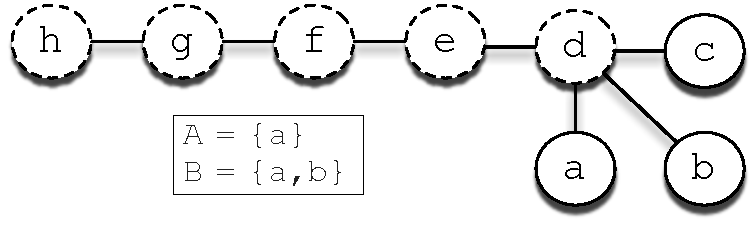
\includegraphics[scale=.75]{figs/submodular-counterexample.pdf}
\caption{Example used in Theorem \ref{thm:submodular1} showing a function defined using our observability rules is not submodular for graphs with zero-injection nodes.  
Nodes with a dashed border are zero-injection nodes and injection nodes have a solid border. For set function $f: 2^X \rightarrow \mathbb{R}$, defined as the number of observed nodes 
resulting from placing a PMU at each $x \in X$, we have $f(A) = f(\{a\}) = 2$ where $\{a,d\}$ are observed, while $f(B) = f(\{a,b\}) = 3$ where $\{a,b,d\}$ are observed.  }
\label{fig:submodular-counter}
\end{figure}


\begin{theorem}
\label{thm:submodular2}
$f$ is a submodular function for graphs, $G_I$, containing only injection nodes.
\end{theorem}

\begin{proof}
Consider a graph $G_I=(V_I,E_I)$ where each $v \in V_I$ is an injection node. Let $A \subseteq B \subseteq V_I$ and $j \in V_I$.  Placing a PMU at $j$ can at most result in the observation of
$j \cup \Gamma(j)$ because we cannot apply O2 in $G_I$ since we have assumed all nodes are injection nodes.
%Since all nodes are injection nodes we cannot use O2 to observe any nodes. and thus nodes can only be observed using O1.  By O1, $j$ and $\Gamma(j)$ are observed.  
We claim that any $x \in j \cup \Gamma(j)$ that is unobserved after placing a PMU at nodes in $B$ is not observed with the PMU placement derived from $A$.  $x$ is unobserved only if 
$x$ has no PMU nor if any $\Gamma(x)$ has a PMU.  Since $A \subseteq B$ and we have assumed $x$ is not observed using $B$, it must be the case that $x$ is not observed under $A$.
%Since $A \subseteq B$, we know that if any $x \in \Gamma(j)$ is unobserved after placing a PMU at nodes in $B$ that $x$ is not observed with the PMU placement derived from $A$. 
Since we have show that all unobserved nodes resulting from PMU placement $B$ must be unobserved under $A$, we conclude that $f(A \cup \{j\}) - f(A) \geq f(B \cup \{j\}) - f(B)$ 
and, therefore, $f$ is submodular for $G_I$.
\end{proof}

%\xxn{Maybe we can show it is a submodular function for certain distributions of zero-injection nodes.}


%\subsection{Example Showing Greedy is not a Submodular Function}
%
%Submodular definition from \footnote{\url{http://theory.stanford.edu/~jvondrak/CS369P-files/lec16.pdf}}.  Denote $f_A(i) = f(A+i) - f(A)$ the marginal value of $i$ with respect
%to $A$.  $f$ is submodular if for all $A \subseteq B \subseteq N$ and $i \in N \setminus B$, 
%$$ f_A(i) \geq f_B(i) $$
%
%
%Execution of {\tt greedy} using Figure \ref{fig:submodular-counter}:
%\begin{enumerate}
%	\item Add PMU to $d$.  As a result, $5$ nodes, $\{a,b,c,d,h\}$, are observed by applying O1 at $d$,  O2 cannot be applied.
%	
%	\item Add PMU to $f$.  As a result, $6$ nodes become observed $\{e,f,g,i,j,k\}$ by applying O1 at $f$ and then repeatedly applying O2 (first at $h$, then at $j$, and finally at $k$)
%
%\end{enumerate}
%
%
%\begin{figure*}[t]
%  \begin{center}
%    \subfigure[The original graph (without any PMUs).]{\label{fig:submodular-counter-step0}
%		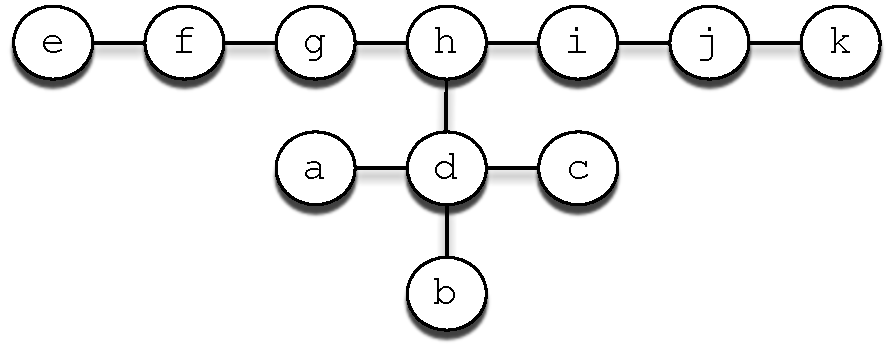
\includegraphics[scale=0.59]{figs/submodular-counterexample-step0.pdf}}
%    \subfigure[Step 1: Placing a PMU at $d$ results in the observation of $5$ nodes, $\{a,b,c,d,h\}$.]{\label{fig:submodular-counter-step1}
%		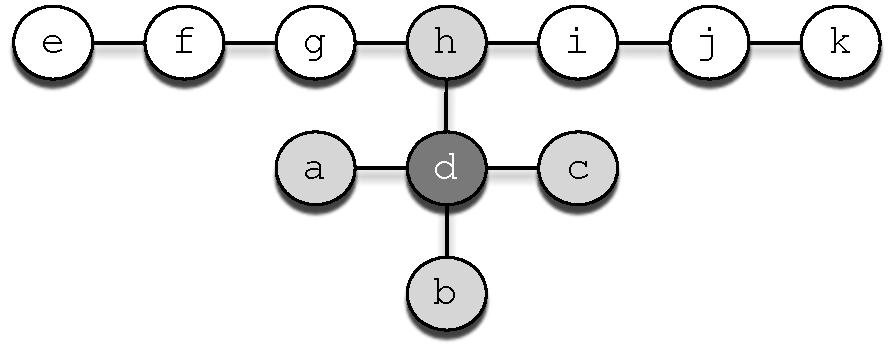
\includegraphics[scale=0.59]{figs/submodular-counterexample-step1.pdf}}
%    \subfigure[Step 2: Placing a PMU at $f$ results in the observation of $6$ nodes, $\{e,f,g,i,j,k\}$.]{\label{fig:submodular-counter-step2}
%		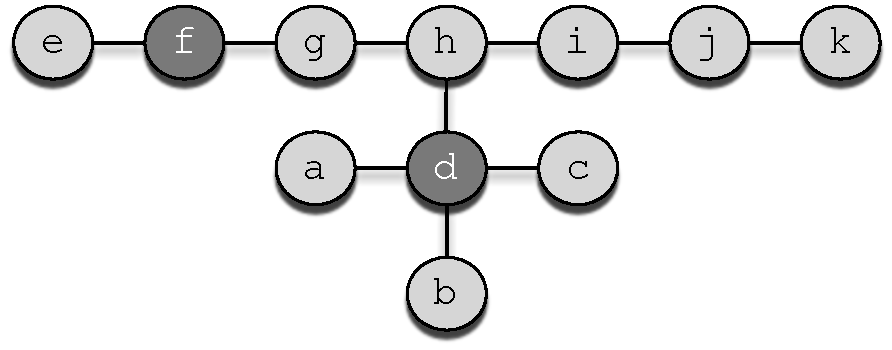
\includegraphics[scale=0.59]{figs/submodular-counterexample-step2.pdf}}
%  \end{center}
%	\caption{Example showing that {\tt greedy} is not a submodular function.} 
%	\label{fig:submodular-counter-old}
%\end{figure*}
%
%\end{comment}


%List of references explaining submodular functions.
%\footnote{Nice definition and examples. \url{http://theory.stanford.edu/~jvondrak/CS369P-files/lec16.pdf}}
%\footnote{Survey paper. \url{http://theory.stanford.edu/~shaddin/papers/submodular_survey.pdf}}
%\footnote{\url{http://en.wikipedia.org/wiki/Submodular_set_function}}
%\footnote{One of the earlier papers on submodular functions. \url{http://www.cs.toronto.edu/~eidan/papers/submod-max.pdf}}


